\documentclass[11pt]{article}
\usepackage{geometry} % Pour passer au format A4
\geometry{hmargin=1cm, vmargin=1cm} % 

% Page et encodage
\usepackage[T1]{fontenc} % Use 8-bit encoding that has 256 glyphs
\usepackage[english,francais]{babel} % Français et anglais
\usepackage[utf8]{inputenc} 

\usepackage{lmodern}
\setlength\parindent{0pt}

% Graphiques
\usepackage{graphicx, float}


% Maths et divers
\usepackage{amsmath,amsfonts,amssymb,amsthm,verbatim}
\usepackage{multicol,enumitem,url,eurosym,gensymb}

% Sections
\usepackage{sectsty} % Allows customizing section commands
\allsectionsfont{\centering \normalfont\scshape}

% Tête et pied de page

\usepackage{fancyhdr} 
\pagestyle{fancyplain} 

\fancyhead{} % No page header
\fancyfoot{}

\renewcommand{\headrulewidth}{0pt} % Remove header underlines
\renewcommand{\footrulewidth}{0pt} % Remove footer underlines

\newcommand{\horrule}[1]{\rule{\linewidth}{#1}} % Create horizontal rule command with 1 argument of height

%----------------------------------------------------------------------------------------
%	Début du document
%----------------------------------------------------------------------------------------

\begin{document}

\textbf{Nom, Prénom :} \hspace{8cm} \textbf{Classe :} \hspace{3cm} \textbf{Date :}\\


\begin{center}
  \textit{Les mathématiques ne sont une moindre immensité que la mer.}  - \textbf{Victor Hugo}
\end{center}

\textit{La présentation, la rédaction et le soin général apportés à la copie sont sur 3 points.}
\begin{itemize}
\item \textsc{Calculer} : 
\item \textsc{Modéliser} : 
\item \textsc{Note} : 
\end{itemize}

\horrule{1px}
\vspace{-1cm}

\subsubsection*{Calculer - \textit{(/3)}}

\begin{center}
  \begin{tabular}{|c||c|c|c|c|c|}
    \hline
    angles &        15\degree &        23\degree &       45\degree &       54\degree & 70\degree \\
    \hline
    $\sin$ & \phantom{azertyuiop} & \phantom{azertyuiop} &\phantom{azertyuiop} &\phantom{azertyuiop} & \phantom{azertyuiop}\\
    \hline 
    $\cos$ & & & & &\\
    \hline
    $\tan$ & & & & &\\
    \hline
  \end{tabular}
\end{center}

\subsubsection*{Modéliser - \textit{(/3)}}

On cherche à calculer le \textbf{?}. Dire si on peut utiliser : $\sin$, $\cos$, $\tan$ ou aucun des trois. \textbf{Justifier}.

  \begin{figure}[H]
    \centering
    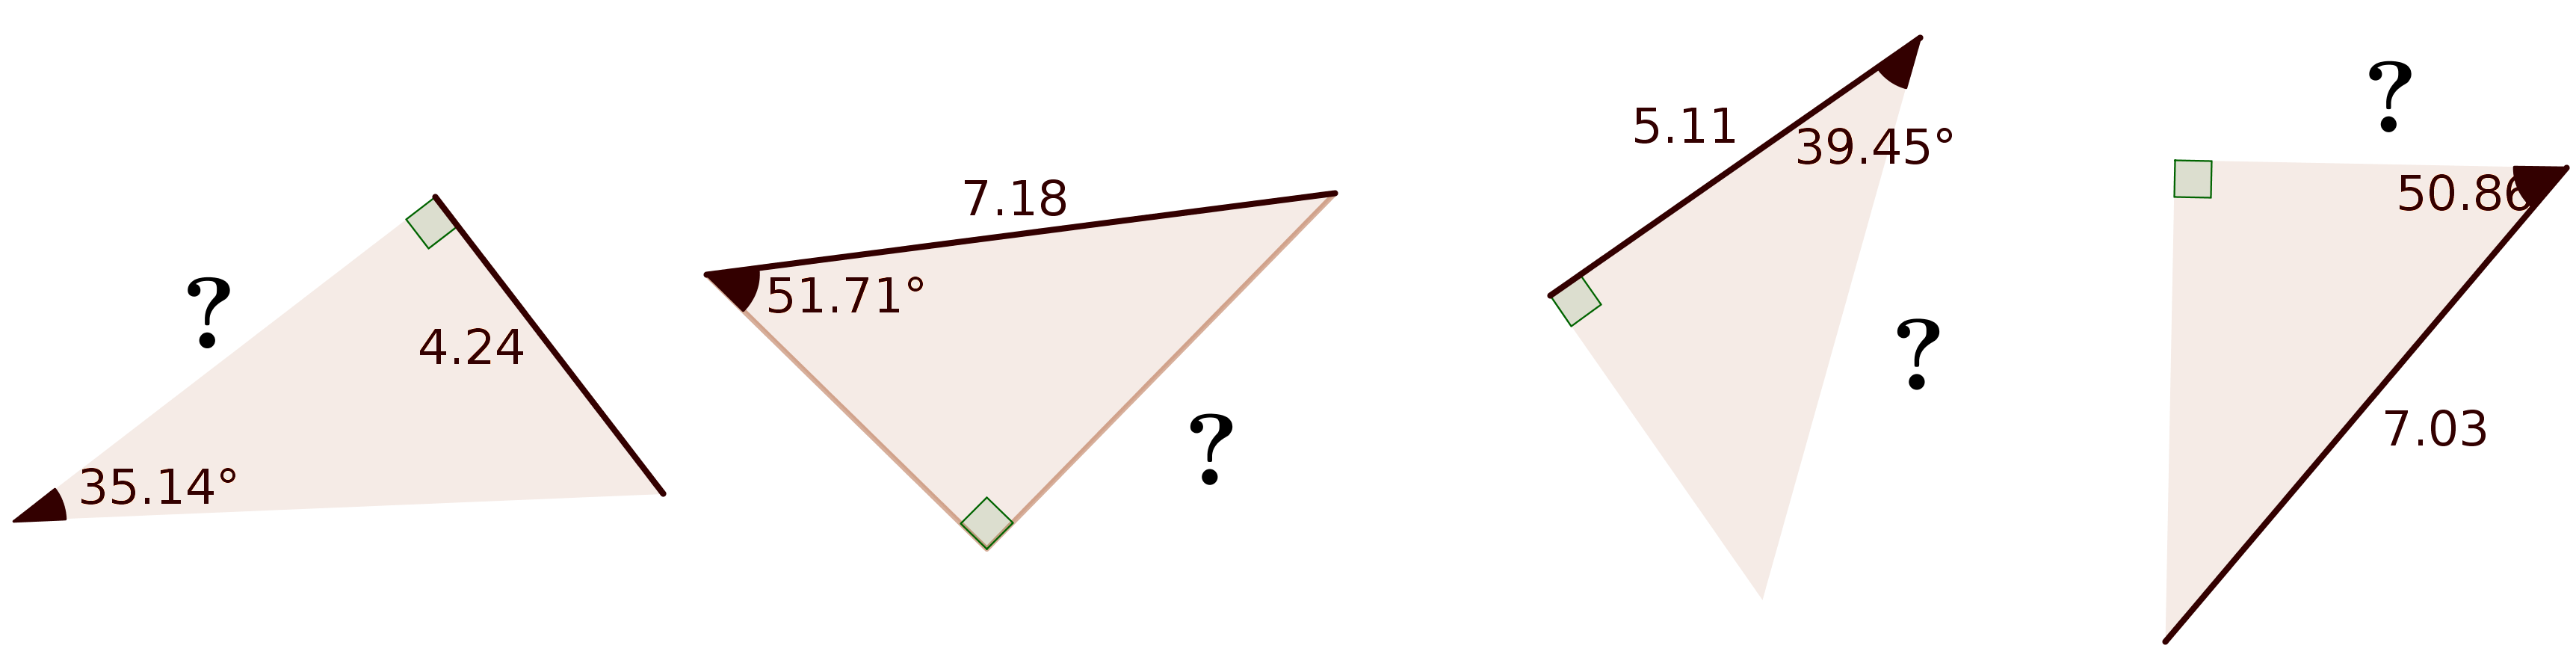
\includegraphics[width=\linewidth]{sources/ch3-trigonometrie/2_trigo_mod.png}
  \end{figure}

\begin{multicols}{2}

\subsubsection*{Exercice - \textit{(/4)}}

\begin{enumerate}
\item[a.] Donner la longueur des trois côtés $AB$, $AC$ et $BC$.
\item[b.] Donner la mesure des trois angles $\widehat{ABC}$, $\widehat{BAC}$ et $\widehat{ACB}$.
\end{enumerate}

  \begin{figure}[H]
    \centering
    \includegraphics[width=0.6\linewidth]{sources/ch3-trigonometrie/2_ex.pdf}
  \end{figure}


\end{multicols}

\subsubsection*{Problème 1 - Du phare aux bateaux  - \textit{(/5)}}
Soit un phare $[AC]$ d'une hauteur 40m. Le premier bateau $B_1$ aperçoit le haut du phare avec un angle de 22\degree. Le deuxième bateau $B_2$ aligné au premier, aperçoit le haut du phare avec angle de 16\degree.

\begin{enumerate}
\item[1a.] Faire un schéma de la situation
\item[1b.] Quelle est la distance séparant les deux bateaux ?
\end{enumerate}

\subsubsection*{Problème 2 - Du bateau aux phares - \textit{(/5)}}

Un navigateur $P$ longe une côté. Il aperçoit deux phares $A$ et $B$. Il sait que $AB = 2km$. Alors qu'il dépasse le premier, il mesure un angle avec le second : $\widehat{APB} = 35\degree$.

\begin{enumerate}
\item[2a.] Faire un schéma de la situation
\item[2b.] Quelle est la distance entre le bateau et chacun des phares ?
\end{enumerate}


\textbf{Bonus : } \textit{Comment s'appelle l'instrument de navigation qui permet de mesurer des angles (et des distances angulaires ?}

\end{document}
